\chapter{Syntax Definition in SDF3}
\chapterlabel{syntax}

In this chapter we study declarative syntax definition with SDF3.
Spoofax takes a \emph{syntax first} approach to language definition.
All semantic operations that we will consider in the rest of the book work on
abstract syntax trees.
Instead of separately describing a grammar, an algebraic signature, and a
mapping from parse trees to abstract syntax trees, an SDF3 syntax definition
describes all three at once. 
Indeed, as we will see, from just an SDF3 syntax definition, we can generate a
range of artifacts including the abstract syntax signature, error recovery
rules, a parser, a mapping from parse trees to abstract syntax trees, a
pretty-printer (mapping from abstract syntax trees to text), syntax
highlighting rules, and folding rules.

Developing and testing a syntax definition in Spoofax are seamless. As
illustrated in \Figure{syntax-dev}, a language and programs in the language can
be edited in the same Eclipse environment, providing a quick turn around time
for changes to the language. The workflow for developing a syntax definition is
simple: make a change to the definition, build the project, and watch the
open editors for SPT tests and example programs being re-analyzed, or invoke
the Spoofax Test Runner to run all tests in the project.

In this chapter we use example project \LanguageRepoRef{LanguageA} as
illustration. The project defines the syntax of a small Java-like language
styled after an assignment that comes with
Krishnamurthi's Programming Languages book \cite{Krishnamurthi2014}.

\begin{figure}[t]
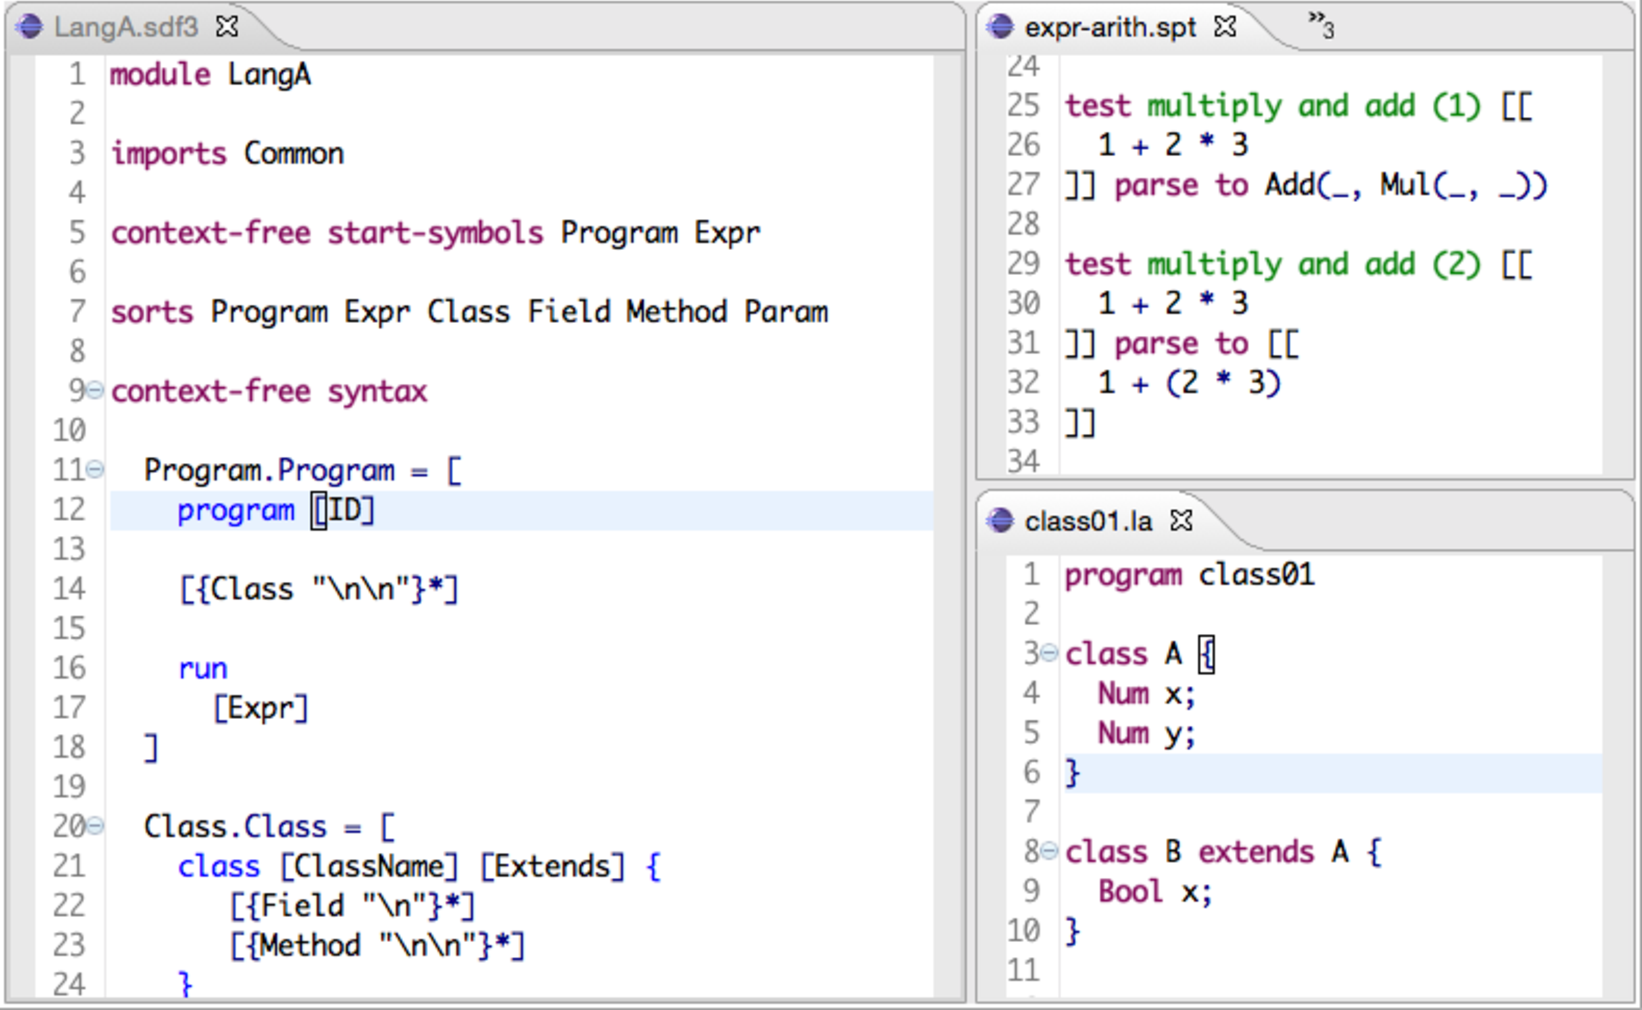
\includegraphics[width=\hsize]{syntax/syntax-dev.pdf}
\caption{Developing and testing syntax definition in the same IDE context.}
\figurelabel{syntax-dev}
\end{figure}


\section{Configuration}

As we indicated in \Chapter{getting-spoofax}, the name that you choose for your
language project is important since it ties a bunch of things in the
configuration of your project together. The main module of the syntax definition
in directory \LanguageFile{LanguageA}{syntax/} has the name of the language.
Thus, we find \LanguageFile{LanguageA}{syntax/LangA.sdf3} in the example
project. Furthermore, the language name is used as prefix of the \texttt{esv}
configuration files in the \LanguageFile{LanguageA}{editor/} directory. The main
configuration module is \LanguageFile{LanguageA}{editor/LangA.main.esv}. It
declares the file extension to be used by programs in the language (\texttt{la})
and the start symbol to be used for such files. By default the start symbol is
set to \texttt{Start}. For \texttt{LanguageA} I have changed it to
\texttt{Program}, since that is the sort in the syntax definition that
represents the content of a file.


\section{Structure of a Syntax Definition}

An SDF3 syntax definition consists of a collection of modules with the following
outline:

\begin{lstlisting}[language=SDF]
module [ModuleName]
imports [ModuleName*]
context-free start-symbols [Symbol*]
[SyntaxSection*]
\end{lstlisting}

A module may import other modules using their declared name. The start symbols
tell the parser with which syntactic sorts to start parsing. While start symbols
may be declared in any module, they are typically declared in the main module of
language. As noted above, when changing the start symbol to something else than
the default \texttt{Start}, this should be changed in the \texttt{main.esv}
module as well.

Let's have a look at the definition of \LanguageRepoRef{LanguageA}. Its main
syntax module defines the sorts \texttt{Program} and \texttt{Expr} as start
symbols and imports the modules \texttt{Programs}, \texttt{Classes}, and
\texttt{Expressions}:

\lstinputlisting[language=SDF]{../languages/LanguageA/syntax/LangA.sdf3}

\section{Concrete and Abstract Syntax}

The programs in \LanguageRepoRef{LanguageA} have a name, then define a list of
zero or more classes, and finally an expression to be executed in the context of
these class definitions. The following is a minimal program in the concrete
syntax of the language that executes the expression \texttt{1} in the context of
no classes:

\lstinputlisting[language=paplj]{../languages/LanguageA/examples/program/program01.la}

Here is the same program in abstract syntax representation:

\lstinputlisting[language=ATerm]{../languages/LanguageA/examples/program/program01.aterm}

The abstract syntax tree is represented as a term with constructors such as
\texttt{Program} and \texttt{Num} creating tree nodes, and strings to represent
lexemes such as identifiers and numbers.

An SDF3 definition defines both the concrete syntax and abstract syntax views of
a language. Here is a (plain version of) the \texttt{Programs} module:

\lstinputlisting[language=SDF]{../languages/LanguageA/syntax/ProgramsPlain.sdf3}

The module imports the syntax of \texttt{Classes} and \texttt{Expressions} and
defines a \emph{context-free syntax production} to define the syntax of
programs. In general, an SDF3 production has the form

\begin{lstlisting}[language=SDF]
  Sort0.C = [lit3 [Sort1] lit2 [Sort2] lit3 ...]
\end{lstlisting}

where \texttt{Sort0} is the non-terminal sort being defined, \texttt{C} is the
abstract syntax tree constructor, and the brackets contain the body of the
production. The body is a sequence of literal symbols, whitespace, and
non-terminal sorts. The notation for productions uses inverted quotation.
Instead of quoting the literal symbols, the sorts are quoted. Thus, a so-called
template production is equivalent to a normal context-free grammar production of
the form:

\begin{lstlisting}[language=SDF]
  Sort0 = "lit3" Sort1 "lit2" Sort2 "lit3"
\end{lstlisting}

Thus, our \texttt{Program} production is equivalent to the context-free grammar
production

\begin{lstlisting}[language=SDF]
  Program = "program" Class* "run" Expr
\end{lstlisting}

defining the concrete syntax notation of programs. By the way, the \texttt{*} in
\texttt{Class*} is the Kleene-star and denotes a sequence of zero or more
strings matching the \texttt{Class} non-terminal sort.

So, what is the use of the constructor? As indicated above, an SDF3 definition
not only defines the concrete syntax (the notation), but also the abstract
syntax, the tree structure representing the underlying structure of the
notation. Thus, for each SDF3 production there is a corresponding algebraic
signature declaration derived by stripping the literals and whitespace from the
production. For the general production form above, we would get the following
constructor declaration:

\begin{lstlisting}[language=Stratego]
  C : Sort1 * Sort2 -> Sort0
\end{lstlisting}

That is, given abstract syntax trees \texttt{t1} and \texttt{t2} of sorts
\texttt{Sort1} and \texttt{Sort2}, respectively, \texttt{C(t1, t2)} is a
well-formed term of sort \texttt{Sort0}.

\Figure{program-sig} shows the Stratego module \texttt{Programs-sig}
with the signature declaration corresponding to our \texttt{Programs} modules.
The constructor declaration for \texttt{Program} describes the structure of the
abstract syntax term that we saw above. Spoofax automatically generates a
signature module in the \texttt{src-gen/signatures} directory of the project for
each SDF3 module.

\begin{figure}[t]
\lstinputlisting[language=Stratego]{../languages/LanguageA/src-gen/signatures/Programs-sig.str}
\caption{Algebraic signature derived from syntax definition module
\texttt{Program}.}
\figurelabel{program-sig}
\end{figure}

The parser generated from the underlying context-free grammar internally
produces a \emph{derivation} (also known as \emph{parse tree}) that uses
context-free grammar productions as node constructors. Following the
correspondence between productions and constructors sketched above, such a parse
tree is converted to an abstract syntax tree automatically.

In the generated editor for your language, you can get the abstract syntax term
of a program using the \texttt{Show Abstract Syntax} entry in the
\texttt{Syntax} menu, as illustrated in \Figure{class01-abstract-syntax}.
This is a great tool for `debugging' your syntax definition. Rather than tracing
the behaviour of the parser, you can inspect how your syntax definition maps
program texts to abstract syntax tree. And if that mapping is not to your
liking, you can adapt the syntax definition, build, and see how the AST is
updated. We will see in \Section{disambiguation} how this tool can be used to
inspect ambiguities in your syntax definition.

\begin{figure}[t]
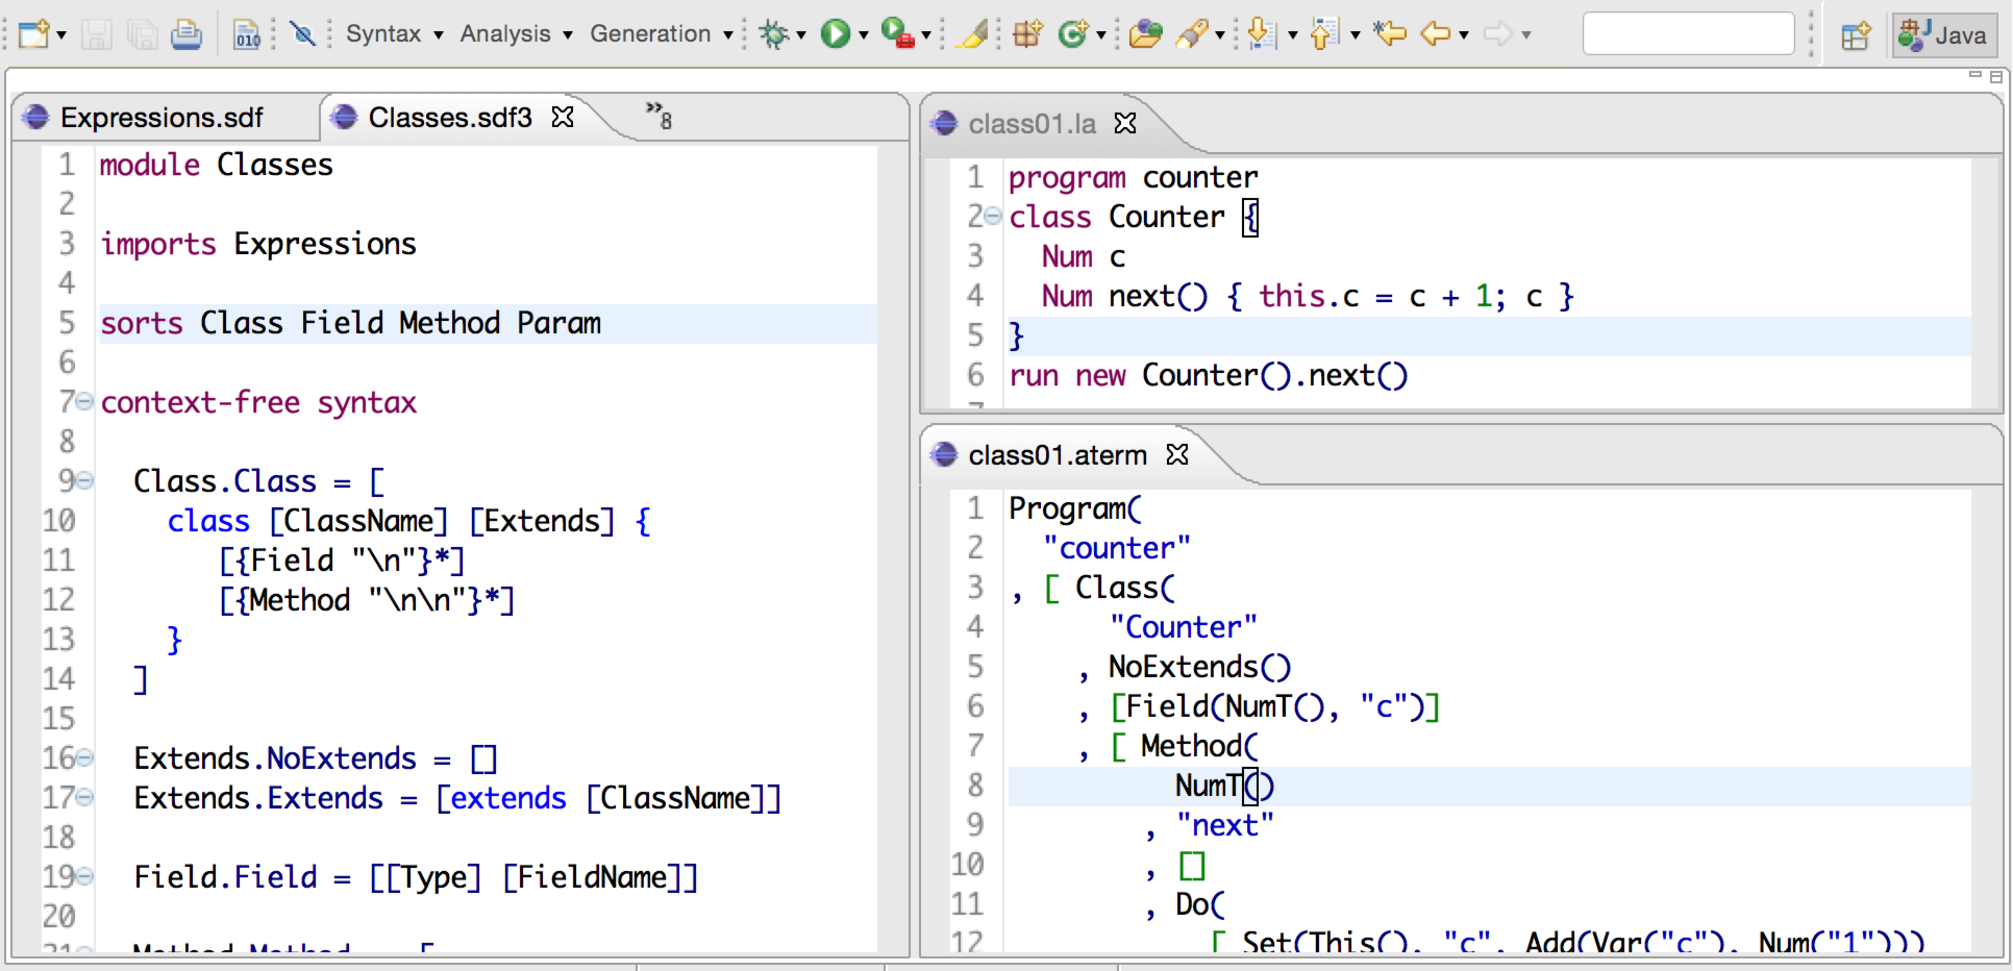
\includegraphics[width=\hsize]{syntax/class01-abstract-syntax.pdf}
\caption{Abstract syntax term \texttt{class01.aterm} for \texttt{class01.la}
obtained using the \texttt{Show Abstract Syntax} entry in the \texttt{Syntax}
menu.}
\figurelabel{class01-abstract-syntax}
\end{figure}
 

We have seen that by extending standard context-free grammar rules with
constructor declarations, we get a parser, an algebraic signature (abstract
syntax tree schema), and a mapping from parse trees to abstract syntax trees for
free. But in addition to constructors, there is another difference between
context-free grammar rules and template productions.

\section{Template Layout}

The inverted quotation templates used as the body of an SDF3 production can be
seen as esthetically pleasing by getting rid of the double quotes for quoting
literals. However, we replace the double quotes by square brackets (or angle
brackets \texttt{<Expr>}), and it requires more of those. And the esthetic
argument will undoubtely run into people with different tastes. So, the argument
for inverted quotation cannot just be esthetics. And indeed it is not.

\begin{figure}[t]\small
\lstinputlisting[language=paplj]{../languages/LanguageA/examples/class/class01.la}
\lstinputlisting[language=ATerm]{../languages/LanguageA/examples/class/class01.aterm}
\caption{Counter class in concrete and abstract syntax.}
\figurelabel{class01.la}
\end{figure}

Consider the concrete and abstract syntax of the \texttt{counter} program in
\Figure{class01.la}.
\Figure{Classes.sdf3} defines the complete syntax of classes, fields, and
methods, except for the syntax of \texttt{Block} that makes the bodies of
methods.
The syntax of a class is defined by the following production:

\begin{lstlisting}[language=SDF]
Class.Class = [
  class [ID] [Extends] {
     [{Field "\n"}*]
     [{Method "\n\n"}*]
  }
]  
\end{lstlisting}

That is, a class has a name, an extends clause, a list of zero
or more fields, and a list of zero or more methods. \texttt{Class} is both the
non-terminal sort and the constructor for class terms. Thus, an abstract syntax
term for class has the form \texttt{Class(name, extends, fields, methods)}.

The production above is equivalent, in terms of parsing and abstract syntax to
the much simpler looking production
  
\begin{lstlisting}[language=SDF]
Class.Class = 
  [class [ID] [Extends] { [Field*] [Method*] }]
\end{lstlisting}

\begin{figure}
\lstinputlisting[language=SDF]{../languages/LanguageA/syntax/Classes.sdf3}
\caption{Syntax of classes with fields and methods.}
\figurelabel{Classes.sdf3}
\end{figure}

What is the use of the multi-line layout of the production above? First, the
production is layed out as one might format a concrete class in a program.
This (arguably) helps the readability of the syntax definition.
For various reasons it is necessary to map an abstract syntax tree back to a
readable textual representation. It is not sufficient to create a flat
concatenation of the literals and lexicals from the production, since that would
result in a single line of text.
It would useful to deduce from the productions of a grammar a mapping to text
that is readable and pretty, i.e. with newlines in the right places and proper
indentation.
No such thing exists, as far as I know. (But it would be great if someone would
come up with an algorithm!) Therefore, in order to produce a useful
pretty-printer, we need to specify where to put the newlines and indentation.
In Stratego/XT \cite{BravenboerKVV08} this was done by generating a default
pretty-printer from the grammar and then manually adapting that to get a good
result. This was tedious work and had to be re-done on each change of the
grammar. As a result, pretty-printers were often out of sync with the grammar.
This is the problem that template productions address.

The layout (whitespace) in the template is used as an example-based
specification for formatting programs. That is, newlines and spaces (for
separation and indentation) in a template are interpreted for \emph{formatting}
of ASTs. For parsing this whitespace is ignored. Or rather, it is not taken as
literally as it is in formatting. Whitespace between two symbols in a production
is taken to signify the presence of optional layout (whitespace and comments)
between those symbols.

Spoofax generates from an SDF3 definition a pretty-printer in the
\texttt{src-gen/pp/} directory of your project. The pretty-printer consists of
Stratego rewrite rules that map an abstract syntax term to a term in the
abstract syntax of the Box formatting language. For example, the generated rule
for \texttt{Class} has the form

\begin{lstlisting}[language=Stratego]
prettyprint-Class :
  Class(t1, t2, t3, t4) -> [..t1'..t2'..t3'..t4'..]
  with t1' := <prettyprint-ID> t1
  with t2' := <prettyprint-Extends> t2
  with t3' := <prettyprint-Field> t3
  with t4' := <prettyprint-Method> t4
\end{lstlisting}

That is, it calls the pretty-print rules for the sub-terms, and combines the
results using combinators of the Box language. I'm omitting the details of the
Box language here, since for most purposes the automatically generated
pretty-printer should be sufficient. If you are curious
have a look at the generated files, such as \texttt{src-gen/pp/Classes-pp.str}.

The generated pretty-printer for your language can be invoked directly from the
\texttt{Format} entry in the \texttt{Syntax} menu of the editors for your
language.
For example, using the pretty-print rules generated from the productions in
\Figure{Classes.sdf3}, the program in \Figure{class01.la} is formatted as
follows:

\lstinputlisting[language=paplj]{../languages/LanguageA/examples/class/class01.pp.la}

\paragraph{Tweaking Formatting}

The formatting of productions can be tweaked by adapting their templates. The
use of newlines and indentation should be obvious from the \texttt{Class}
example. We can learn some further techniques from the \texttt{Method}
production in \Figure{Classes.sdf3}:

\begin{lstlisting}[language=SDF]
  Method.Method =  [
  	[Type] [ID]([{Param ", "}*]) [Block]
  ]
\end{lstlisting}

The separation of symbols by a space in the template means that they will be
separated by a space in the formatted text as well. But the \emph{lack of a
space separation} is significant as well. For example, this template specifies
that the name of the method and the subsequent parenthesis should \emph{not} be
separated by a space, nor should there be spaces after the open parenthesis and
before the closing parenthesis of the parameter list. However, following good
typographic practice, the commas in the list of parameters \emph{should} be
followed by a space.

By the way, note that the notation \sdfcode{\{Param ","\}*} denotes a sequence
of zero or more \texttt{Param}s \emph{separated by} commas. Compare this to the
usual way to encode lists with separators in grammars.

\paragraph{Code Completion}

The layout information in templates is not just useful for pretty-printing, but
is also applied in the production of code completion templates. For each
(template) production, Spoofax generates a template such as the following for
the \texttt{Class} rule (in the \texttt{src-gen/completions/Classes-esv.esv}
module):

\begin{lstlisting}[language=ESV]
completion template Class : "class ID Extends { }" =
  "class " <ID:ID> " " <Extends:Extends> " {\n\t" 
     (cursor) "\n}" (blank)  
\end{lstlisting}

The layout directives in the template (space, newlines, tabs) are derived from
the layout in the production template.

Given such templates, the editor for your language supports syntactic code
completion. When hitting the Control-Space key combination in an editor, the
editor proposes a list of possible completions at that point in the program.

\paragraph{Discussion: User-Defined Preferences}

Template-based formatting for a language hard-wires the definition of
formatting. Possibly, you might want to provide the users of your language with
the possibility of adapting the formatting to their taste. This scenario is
currently not supported by Spoofax. It is conceivable that such a feature could
use the template-based preferences as language defaults and as an indication of
the choice points for such a preference dialog.

However, one could also adopt 
\href{http://blog.golang.org/go-fmt-your-code}{the point of view} 
of the \href{http://golang.org/}{Go language} and require all programs committed
to version control to be formatted with the same standardized formatting rules.
This ensures that all programs look the same and no time is wasted on petty
formatting wars. Of course, this requires the language is suitable for such
standardized formattting; for (functional) languages with large expressions,
good formatting often requires insight in the meaning of the program. 

\paragraph{Summary}

To summarize, \Figure{Classes.sdf3} illustrates the basic features that 
we have learned about SDF3 so far:

\begin{itemize}
  \item Modules divide a syntax definition in (reusable, importable) parts.
  \item The syntax of a non-terminal is defined by multiple productions, one for
  each alternative.
  \item A production defines the name of the constructor used in the
  construction of the corresponding abstract syntax tree node.
  \item The template body of a production uses inverted quotation to capture a
  program pattern.
  \item Sequences and sequences with separators are concisely
  captured by the \sdfcode{A*} and \sdfcode{\{A sep\}*} symbols.
  \item The whitespace in a template body informs the generation of pretty-print
  and code completion rules.
\end{itemize}


\section{Expression Syntax}

Let's try to apply these features to the definition of expression syntax.

\begin{lstlisting}[language=SDF]
module LangA
imports Common
context-free start-symbols Program Expr
context-free syntax
  Exp.Var = ID
  Exp.Mul = [[Exp] * [Exp]]
  Exp.Add = [[Exp] + [Exp]]
\end{lstlisting}

templates \cite{VollebregtKV12}


\section{Disambiguation}
\sectionlabel{disambiguation}

\begin{lstlisting}[language=SDF]
module 
context-free syntax
  Exp.Var = ID
  Exp.Mul = [[Exp] * [Exp]] {left}
  Exp.Add = [[Exp] + [Exp]] {left}
context-free priorities
  Exp.Mul > Exp.Add
\end{lstlisting}

\section{Lexical Syntax}

So far, we have completely ignored the lexical syntax of languages. We have used
the \texttt{ID} and \texttt{INT} sorts to introduce identifiers and integer
literals in our language, but have not looked at their definition, nor have we
looked at the specification of whitespace and comments. We got away with that by
importing the \texttt{Common} module that the Spoofax wizard includes in the
\texttt{syntax/} directory of a new project. It defines the lexical syntax of
common lexical categories such as identifiers, strings, whitespace, and
comments. For many languages, it will suffice to use these. But if you need to
tweak the lexical syntax, or need to add new categories then it is useful to
know how it is done. Fortunately, it is not difficult at all. 

\begin{figure}
\lstinputlisting[language=SDF]{../languages/LanguageA/syntax/Common.sdf3}
\caption{The \texttt{Common} SDF3 module included in new Spoofax projects,
defining the syntax of common lexical categories.}
\figurelabel{Common.sdf3}
\end{figure}

\Figure{Common.sdf3} contains the content of module \texttt{Common}.
The lexical syntax section contains productions for lexical syntax sorts.
The productions are general context-free grammar productions of the form
\texttt{[NT] = [Symbol*]} defining an alternative for the non-terminal
\texttt{NT}. The difference between lexical syntax productions and context-free
syntax productions is that the former typically do not use template notation,
but rather a plain sequence of symbols (but they may use templates).
Furthermore, lexical syntax productions do not define a constructor since their
parse tree is flattened to a single string when producing an abstract syntax
tree.

\paragraph{Character Classes}

In addition to string literals such as \sdfcode{"class"} that we encountered in
context-free productions, lexical production also use \emph{character classes}
that denote the choice between a range of characters. For example, the
production for identifiers

\begin{lstlisting}[language=SDF]
ID = [a-zA-Z] [a-zA-Z0-9]* 
\end{lstlisting}

uses the character classes \sdfcode{[a-zA-Z]} and \sdfcode{[a-zA-Z0-9]}.

\paragraph{Layout Separation}

The key difference between lexical syntax and context-free syntax is that the
symbols of context-free productions are separated by optional layout. That is, a
context-free syntax production such as

\begin{lstlisting}[language=SDF]
Exp.Add = Exp "+" Exp 
\end{lstlisting}

is sugar for

\begin{lstlisting}[language=SDF]
Exp.Add = Exp LAYOUT? "+" LAYOUT? Exp 
\end{lstlisting}

which states that the symbols of an addition can be separated by whitespace or
comments. This desugaring is \emph{not} applied to lexical syntax productions,
which entails that the symbols making up a lexeme cannot be separated by layout.

\paragraph{Disambiguation}

\section{Error Recovery}

\cite{JongeKVS12}


\section{Further Reading}

The goal of declarative syntax definition is to enable language designers to
think about syntax in terms of the (tree) structures underlying programs instead
of in terms of parsing algorithmics \cite{KatsVW10}.
SDF3 is the third generation Syntax Definition Formalism that takes declarative
syntax definition as its guiding design principle.
The original Syntax Definition Formalism SDF \cite{HeeringHKR89} introduced the
specification of lexical syntax and context-free syntax in a single formalism,
the adaptation of Tomita's generalized LR-parsing algorithm to programming
language grammars \cite{Rekers1992,Tomita85}, the automatic mapping of parse
trees to compact abstract syntax trees, and disambiguation by means of
associativity and priorities.
The second generation SDF2 truly integrated lexical and context-free syntax by
using a single formalism (context-free grammar productions) for the
specification of both \cite{Vis97.thesis,Visser-1997-SDF} and supporting this by
the introduction of scannerless, generalized (LR) parsing~\cite{Vis97.sglr}.
This required the introduction of lexical disambiguation techniques such as
reject productions and follow restrictions. The third generation SDF3 introduced
the notion of template productions for the derivation of pretty-printers and code completion schemas \cite{VollebregtKV12}.
Furthermore, SDF3 first formalized the declaration of abstract syntax tree
constructors as part of production rules and their use for the specification of
priorities.


Pretty-printing using the box language is implemented in the
\href{http://releases.strategoxt.org/docs/api/libstratego-gpp/stable/docs/}{libstratego-gpp}
Stratego library, based on the work of Merijn de Jonge \cite{Jonge02}. The
general approach of generating pretty-printers was first explored in the ASF+SDF
MetaEnvironment \cite{BV94,BrandV96}.

\cite{JongeV11}: An Algorithm for Layout Preservation in Refactoring
Transformations

\cite{BravenboerTV06}: syntax of AspectJ

\cite{KlintV94,BrandSVV02}: disambiguation filters


\cite{BravenboerV08}: Parse table composition
